\chapter{The Su-Schrieffer-Heeger Model}
Basic concepts of topological insulatrors va a concrete system: the Su-Schrieffer-Heeger (SSH) model describes spinless fermions hopping on a one-dimensional lattice with staggered hopping amplitudes.
\begin{itemize}
    \item Single-particle Hamiltonian
    \item Bulk and boundary
    \item chiral symmetry
    \item adiabatic equivalence
    \item topological invariants
    \item bulk-boundary correspondence
\end{itemize}

\section{The SSH Hamiltonian}\label{sec:1.1}
The Su-Schrieffer-Heeger (SSH) model describes electron hopping on a chain with staggered hopping amplitudes.
Interactions between electrons are neglected, so the single-particle Hamiltonian:
\begin{equation}
    \hat{H} = v \sum_{m=1}^N \left( \ket{m,B}\bra{m,A} + h.c. \right) + w \sum_{m=1}^{N-1} \left( \ket{m+1,A}\bra{m,B} + h.c. \right)
    \label{eq:1.1}
\end{equation}
\begin{figure}
    
\includegraphics[width=0.9\textwidth]{./fig/ssh_chain_bulkedge.png}
    \caption{Geometry of the SSH model.}
    \label{fig:1.1}
\end{figure}
We \textbf{interested} in the dynamics of fermions in and around the ground state of the SSH model at zero temperature and zero chemical potential, where all negative energy eigenstates of the Hamiltonian are singly occupied\marginnote{As will show later, due to the absence of onsite potential term, there are $H$ such occupied states.
This situation--called half filling--is characteristic of the simplest insulators such as polyacetylene, where each carbon atom brings one conduction electron, and so we find one particle of each spin type per unit cell.}.

\subsection{External and Internal Degrees of Freedom}\label{sec:1.1.1}
A practical representation which separate the external (unit cell index $m$) and internal (sublattice index $\alpha$) degrees of freedom.
Using tensor product basis,
\begin{equation}
    \ket{m,\alpha} \to \ket{m} \otimes \ket{\alpha} \in H_{external} \otimes H_{internal}
    \label{eq:1.3}
\end{equation}
with $m=1, \dots, N$, and $\alpha \in \lbrace A, B\rbrace$.

The Hamiltonian reads
\begin{equation}
    H = v \sum_{m=1}^N \ket{m}\bra{m} \otimes \sigma_x + w \sum_{m=1}^{N-1} \left( \ket{m+1}\bra{m} \otimes \frac{\sigma_x + \i\sigma_y}{2} + h.c. \right)
    \label{eq:1.5}
\end{equation}

\section{Bulk Hamiltonian}\label{sec:1.2}
The physics in the bulk, the long central part of the system, should not depend on how the edges are define, so we can use periodic boundary conditions.

\subsection{Bulk Momentum-Space Hamiltonian}\label{sec:1.2.1}
Applying Bloch's theorem, and introducing plane wave basis states \textbf{only for external degree of freedom}
\begin{equation}
    \ket{k} = \frac{1}{\sqrt{N}} \sum_{m=1}^N e^{imk} \ket{m}, ~ ~ ~ k\in \lbrace \delta_k, \dots, N\delta_k \rbrace ~ ~ ~with~  \delta_k = \frac{2\pi}{N}
    \label{eq:1.8}
\end{equation}
The Bloch eigenstates reads
\begin{equation}
    \ket{\Psi_n(k)} = \ket{k} \otimes \ket{u_n(k)};~ ~ ~ \ket{u_n(k)} = a_n(k) \ket{A} + b_n(k) \ket{B}
    \label{eq:1.9}
\end{equation}
The vectors $\ket{u_n(k)} \in H_{internal}$ are eigenstates of the \textit{bulk momentum-space Hamiltonian} $H(k)$ defined as
\begin{equation}
    H(k) = \bra{k} H_{bulk} \ket{k} = \sum_{\alpha,\beta\in \lbrace A,B \rbrace} \bra{k,\alpha} H_{bulk} \ket{k,\beta} \cdot \ket{\alpha} \bra{\beta}
    \label{eq:1.10}
\end{equation}
\begin{equation}
    H(k) \ket{u_n(k)} = E_n(k) \ket{u_n(k)}
    \label{eq:1.11}
\end{equation}

\subsection{Periodicity in Wavenumber}\label{se:1.2.2}
Although Eq.~\ref{eq:1.9} has a lot to do with the \textit{continuous-variable Bloch theorem}, $\Psi_{n,k}(x) = e^{ikx}u_{n,k}(x)$, this correspondence is not direct.
The internal degree of freedom would play the role of the coordinate within the unit cell.
The function $u_{n,k}(x)$ is periodic in real space but not in Brillouin zone.
\begin{eqnarray}
    u_{n,k}(x+1) &=&u_{n,k}(x) \\
    u_{n,k+2\pi}(x+1) &\neq& u_{n,k}(x)
\end{eqnarray}
The Fourier transform acts only on the external degree of freedom, we have the periodicity in the Brillouin zone in \textbf{discredited system}
\begin{equation}
    H(k+2\pi) = H(k);~ ~ ~ \ket{u_n(k+2\pi)} = \ket{u_n(k)}
    \label{eq:1.12}
\end{equation}
The Schrodinger equation defining the matrix of the bulk momentum space Hamiltonian reads
\begin{equation} \label{eq:1.14}
    H(k) = \begin{pmatrix}
        0 & v+we^{ik} \\
        v+w^{-ik} & 0
    \end{pmatrix}
    ~ ~ ~
    H(k)
    \begin{pmatrix}
        a(k)\\
        b(k)
    \end{pmatrix}
    = E(k)
    \begin{pmatrix}
        a(k)\\
        b(k)
    \end{pmatrix}
\end{equation}

\subsection{The Hopping Is Staggered to Open a Gap}\label{sec:1.2.3}
The dispersion of the bulk read from \eqref{eq:1.14},
\begin{equation}
    E(k) = \pm \sqrt{v^2 +w^2 -2vw \cos k}
    \label{eq:1.15}
\end{equation}
There is an energy gap of $\Delta$ separate the lower and upper band
\begin{equation}
    \Delta = \min_k E(k) = \abs{v-w}
    \label{eq:1.16}
\end{equation}

\subsection{Information Beyond the Dispersion Relation}\label{sec:1.2.4}
Stationary states do not only have an energy and wavenumber eigenvalue, but also an internal structure, represented by the components of the corresponding vector $\ket{u_n(k)} \in H_{internal}$.

For any two band model, the Hamiltonian reads
\begin{equation}
    H(k) = d_0(k) \sigma_0 + \hat{d}(k) \hat{\sigma}
    \label{eq:1.17}
\end{equation}
The internal structure of the eigenstates is given by the direction in which the vector $\hat{d}(k)$ points.

As the wavenumber runs through the Brillouin zone, the path of $d_{xy}$ form a close a circle centered at $(v,0)$.
For more general 2-band insulators, this path need not to be a circle, but it needs to be a closed loop due to the periodicity of the bulk momentum-space Hamiltonian, \eqref{eq:1.12}, and to describe an insulator it needs to avoid the origin.
The topology of this loop can be characterized by an integer, the \textbf{bulk winding number} $\nu$.
This counts the number of times the loop winds around the origin of $d_{x-y}$ plane as shown in Fig.~\ref{fig:1.2}.

\begin{figure*}
    \center
    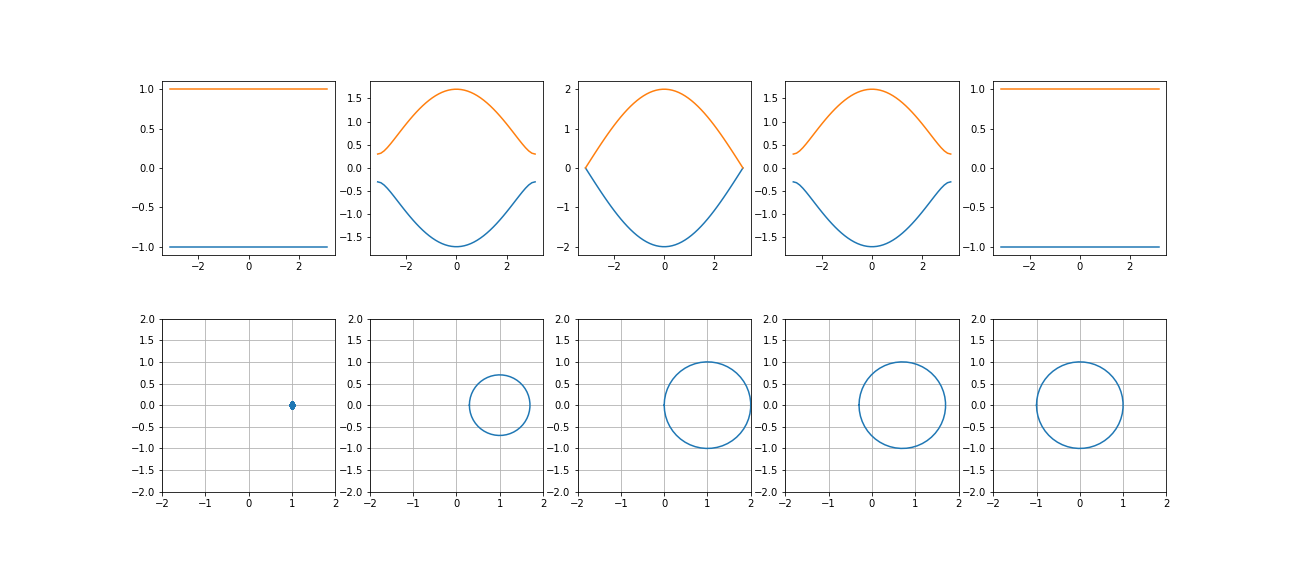
\includegraphics[width=0.9\textwidth]{./fig/fig1-2.png}
    \caption{Eigenvalue and $d_{x-y}$ plot result. From left to right: $v=1,w=0$; $v=1,w=0.7$; $v=1,w=1$; $v=0.7,w=1$; $v=0,w=1$.}
    \label{fig:1.2}
\end{figure*}

\section{Edge States} \label{sec:1.3}
The distinction between bulk and edge is not sharply defined, it describes the behaviour of energy eigenstates in the thermodynamic limit.
One usually can distinguish edge states and bulk states by their localized/delocalized behaviour in the thermodynamic limit.

\subsection{Fully Dimerized Limits} \label{sec:1.3.1}
The SSH model becomes particularly two fully dimerized case: $v=1, w=0$ and $v=0, w=1$.

\newthought{The Bulk in the Fully Dimerized Limits Has Flat Bands}\\
In the fully dimerized limits, one can choose a set of energy eigenstates which are restricted to one dimer each.
These consist of the even ($E=1$) and odd superpositions of the two sites forming a dimer.

In first case $v=1, w=0$ case, we call \textit{trivial},
\begin{equation}
    \hat{H} (\ket{m,A} \pm \ket{m,B}) = \pm( \ket{m,A} \pm \ket{m,B})
    \label{eq:1.19}
\end{equation}

In another case $v=0, w=1$, which is \textit{topological}, each dimer is shared between two neighboring unit cells,
\begin{equation}
    \hat{H} (\ket{m,B} \pm \ket{m+1,A}) = \pm( \ket{m,B} \pm \ket{m+1,A})
    \label{eq:1.20}
\end{equation}

\newthought{The Edges in the Fully Dimerized Limit Can Host Zero Energy States}\\
In trivial case, all energy eigenstates of the SSH chain are given by the formulas of the bulk \eqref{eq:1.19}.
In the topological case, system have more energy eigenstates than those listed in \eqref{eq:1.20}.
Each end of the chain hosts a single eigenstate at zero energy,
\begin{equation}
    \hat{H} \ket{1,A} = \hat{H} \ket{N,B} = 0
    \label{eq:1.21}
\end{equation}
These eigenstates have support on one site only.
Their energy is zero because onsite potential are not allowed in the SSH model.
There are the simplest examples of \textit{edge states}.

\subsection{Moving Away from the Fully Dimerized Limit}\label{sec:1.3.2}
We examine what happens to the edge states as one move away from the fully dimerized limit by increasing $v$.
The spectra, Fig.~\ref{fig:1.4}, reveal that the energies of the edge states remain very close to zero energy.
\begin{figure*}
    \center
    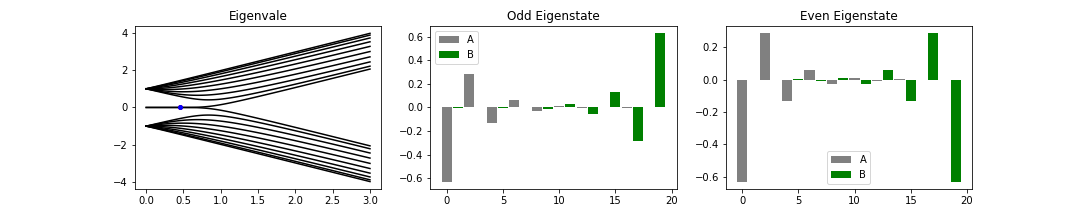
\includegraphics[width=0.9\textwidth]{./fig/fig1-4.png}
    \caption{Eigenenergy and eigenstate of a finite-size SSH model.}
    \label{fig:1.4}
\end{figure*}

The wavefunctions of almost-zero-energy edge states have to be exponentially localized at the left/right edge, because the zero energy is in the bulk band gap.

Some properties about these edge state: the almost-zero-energy eigenstates are odd and even superpositions of states localized exponentially on the left and right edge.
This is a result of exponentially small overlap between the left and right edge state.
Another property of the left (right) edge states, is the right edge state has nonvanishing componenets only on the $A$ sublattice while the left edge estate on teh $B$ sublattices.

\section{Chiral Symmetry} \label{sec:1.4}
One say that a Hamiltonian $H$ has a sysmmetry represented by a \textbf{unitary operator} $U$ if
\begin{equation}
    \hat{U}\hat{H}\hat{U}^\dagger = \hat{H}
    \label{eq:1.22}
\end{equation}

This can be understood as a superselection rule: if we partition the Hilbert space into different sections, i.e., eigenspace of $U$, labeled by the corresponding eigenvalues, then the dynamics as defined by $H$ can be regarded separately in each sector.

\subsection{A Different Type of Symmetry} \label{sec:1.4.2}
In condensed matter physics, the word "symmetry" is used in different sense.
The system with Hamiltionian has \textbf{chiral symmetry} if
\begin{equation}
    \hat{\Gamma}\hat{H}\hat{\Gamma}^\dagger = -\hat{H}
    \label{eq:1.23}
\end{equation}
with an operator $\Gamma$ is not only unitary, but have some other criteria as well.

First, the chiral symmetry operator has to be unitary and Hermitian, $\Gamma^\dagger = \Gamma$, which can be written as
\begin{equation}
    \hat{\Gamma}^\dagger \hat{\Gamma} = \hat{\Gamma}^2 = 1
    \label{eq:1.24}
\end{equation}
This means $\Gamma\Gamma H \Gamma\Gamma = H$.
This means we just leave room for the chiral symmetry operator to square to a state independent pahse, $\Gamma^2 = e^{i\phi}$.
However, this can be get rid of by the redefinition of the  operator $\Gamma \to e^{-i\phi/2}\Gamma$.

Second, it is also required that the sublattice operator $\hat{\Gamma}$ be local.
The system is assumed to consist of unit cell, and matrix elements of $\Gamma$ between sites from different unit cells should vanish\footnote{In SSH chain, this means $\bra{m,\alpha} \hat{\Gamma} \ket{m',\alpha'}=0$}.
Then it is simple to demand the sublattice operator act in the same way in each unit cell, its action represented by a unitary operator $\hat{\gamma}$ acting on the internal Hilbert space of one unit cell,
\begin{equation}
    \hat{\Gamma} = \hat{\gamma} \oplus \hat{\gamma} \oplus \dots \oplus \hat{\gamma} =  \oplus_{m=1}^N \hat{\gamma}
    \label{eq:1.26}
\end{equation}

The third requirement, is that the chiral symmetry has to be robust.
Consider a set of all realizations of disorder $\Theta$, we have
\begin{equation}
    \forall \xi \in \Theta: ~ \hat{\Gamma} \hat{H}(\xi) \hat{\Gamma} = - \hat{H}(\xi)
    \label{eq:1.27}
\end{equation}
with the symmetry operator $\hat{\Gamma}$ independent of the pararmeters $\xi$.
This is robustness of the chiral symmetry.

\subsection{Consequences of Chiral Symmetry for Energy Eigenstates}\label{sec:1.4.3}
Chiral symmetry is also called \textbf{sublattice symmetry}.
One can define orthogonal sublattice porjectiors $P_A$ and $P_B$ as
\begin{equation}
    \hat{P}_A = \frac{1}{2} \left(\mathbb{1} + \hat{\Gamma} \right) ~ ~ ~ \hat{P}_B = \frac{1}{2} \left(\mathbb{1} - \hat{\Gamma} \right)
    \label{eq:1.28}
\end{equation}
where $P_A + P_B = \mathbb{1}$ and $P_A P_B = 0$.
The sublattice symmetry, \eqref{eq:1.23}, can be written in an equivalent form by requiring that the Hamiltonian induce no transitions from any site on one sublattice to any site on the same sublattice,
\begin{equation}
    \hat{P}_{A(B)} \hat{H} \hat{P}_{A(B)} = 0; ~ ~ ~ \hat{H} = \hat{P}_A \hat{H} \hat{P}_B + \hat{P}_B \hat{H} \hat{P}_A
    \label{eq:1.29}
\end{equation}
This is an alternative and equivalent way of defining chiral symmetry.

\newthought{Symmetric Spectrum}\\
The spectrum of a chiral symmetric Hamiltonian is symmetric.

For $E_n \neq 0$, the states $\ket{\psi_n}$ and $\Gamma\ket{\psi_n}$ are eigenstates with different energy and therefore have to be orthogonal.
his implies that every nonzero energy eigenstate of $H$ has equal support on both sublattice\footnote{$0 = \bra{\psi_n} \hat{\Gamma} \ket{\psi_n} = \bra{\psi_n}P_A\ket{\psi_n}- \bra{\psi_n} P_B \ket{\psi_n}$}.

For $E_n = 0$, zero energy eigenstates \textbf{can be chosen} to have support on only one sublattice\footnote{This means the state can be only choose on A or B},
\begin{equation}
    \label{eq:1.32}
    \hat{H}\ket{\psi_n} = 0 : ~ ~ ~ \hat{H} \hat{P}_{A/B} \ket{\psi_n} = \hat{H} \left( \ket{\psi_n} \pm \hat{\Gamma}\ket{\psi_n}\right) = 0
\end{equation}
These projected zero-energy eigenstates are eigenstates of $\Gamma$, and therefore are chiral symmetric partners of themselves\footnote{$\hat{P}_A \ket{\psi_n} = \hat{\Gamma} \ket{\psi_n}$ }.

\subsection{Sublattice Projectors and Chiral Symmetry of the SSH Model}\label{sec:1.4.4}
The Hamiltonian of SSH model, \eqref{eq:1.1}, is bipartite: the Hamiltonian includes no transitions between sites with the sam sublattice index.
The projectors to sublattices read
\begin{equation}
    \hat{P}_{A/B} = \sum_{m=1}^N \ket{m,A(B)} \bra{n,A(B)}
    \label{eq:1.33}
\end{equation}
Chiral symmetry is represented by the sublattice operator,
\begin{equation}
    \hat{\Sigma}_z = \hat{P}_A - \hat{P}_B
    \label{eq:1.34}
\end{equation}

The chiral symmetry of the SSH model is a restatement of the fact that the Hamiltonian is bipartite,
\begin{equation}
    \hat{P}_A \hat{H} \hat{P}_A = \hat{P}_B \hat{H} \hat{P}_B = 0 \to \hat{\Sigma}_z \hat{H} \hat{\Sigma}_z = - \hat{H}
    \label{eq:1.35}
\end{equation}

\subsection{Consequence of Chiral Symmetry: Bulk Winding Number for the SSH Model}\label{sec:1.4.5}
Consider the bulk momentum-space Hamiltonian $H(k) = \mathbf{d}(k) \hat{\sigma}$.

The path of the endpoint of $\mathbf{d}(k)$ , as the wavenumber goes through the BZ, is a closed path on $d_x$, $d_y$ plane.
This path has to avoid the origin, if not, the gap would close and it would not be an insulator.
\textit{Because of the chiral symmetry, the vector $\mathbf{d}(k)$ is restricted on the $d_xd_y$ plane.}
\begin{equation}
    \hat{\sigma}_z \hat{H}(k) \hat{\sigma}_z = - \hat{H}(k) ~ ~ ~ \to ~ ~ ~ d_z(k) = 0 \label{eq:1.36}
\end{equation}

The endpoint of $\mathbf{d}(k)$ is a closed, directed loop on the plane, and thus has a well defined integer winding number about the origin.

\newthought{Winding Number as an Integral}

The winding number can be written as a compact formula using the unit vector $\tilde{\mathbf{d}} = \mathbf{d}/\abs{\mathbf{d}}$.
With the case $\abs{\mathbf{d}(k)} \neq 0$, the winding number $\nu$ is give by
\begin{equation}
    \nu = \frac{1}{2\pi} \int_{-\pi}^{\pi} \left( \tilde{\mathbf{d}}(k) \times \frac{d}{dk} \tilde{\mathbf{d}}(k) \right)_z dk
    \label{eq:1.38}
\end{equation}

To calculate $\nu$ directly from the bulk momentum-space Hamiltonian, note that it is off-diagonal \textbf{in the basis of eigenstates of the chiral symmetry operator $\sigma_z$}
\begin{equation}
    H(k) =
    \begin{pmatrix}
        0 & h(k) \\
        h^*(k) & 0
    \end{pmatrix};
    ~ ~ ~ h(k) = d_x(k) - id_y(k) \label{eq:1.39}
\end{equation}
Then the winding number can be written as
\begin{equation}
    \nu = \frac{1}{2\pi} \int_{-\pi}^{\pi} dk \frac{d}{dk} \log h(k)    \label{eq:1.40}
\end{equation}

\newthought{Winding Number of the SSH Model}

For the SSH model, the winding number is either $0$ or $1$, depending on the parameters.
To change the winding number $\nu$ of the SSH model, we need to
\begin{itemize}
    \item pull the path of $\mathbf{d}(k)$ through the origin in the $d_x$, $d_y$ plane. \textbf{Requires closing the bulk gap}
    \item lift it out the plane and put it back on the plane at a different position. \textbf{Requires breaking chiral symmetry}
\end{itemize}

\section{Number of Edge States as Topological Invariant}\label{sec:1.5}
An insulator Hamiltonian is \textbf{adiabatically} deformed if
\begin{itemize}
    \item its parameters are changed continuously
    \item the important symmetries of the system are maintained
    \item the bulk gap around $E=0$ remain open
\end{itemize}

\subsection{Adiabatic Equivalence of Hamiltonians}\label{sec:1.5.1}
To insulating Hamiltonians are said to be \textit{adiabatically equivalent} or \textit{adiabatically connected} if there is an adiabatic deformation connecting them that represents the important symmetries.
The phase diagram of SSH model is shown in Fig.~\ref{fig:1.7}.
\begin{marginfigure}
    \center
    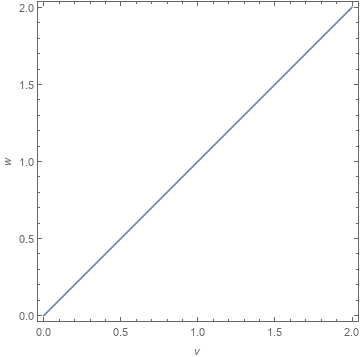
\includegraphics[width=0.85\textwidth]{fig/fig1-7.png}
    \caption{Phase diagram of the SSH model. Gap open case happen at $v=w$. Trivial case $v>w$, intracell hoping is bigger.}
    \label{fig:1.7}
\end{marginfigure}
Two points are adiabatically equivalent if the connection can avoid crossing the middle line

\subsection{Topological Invariant}\label{sec:1.5.2}
We call an integral number characterizing an insulating Hamiltonian a \textit{topological invariant}, if it cannot change under adiabatic deformations.
Two properties of the topological invariant:
\begin{itemize}
    \item it is only well defined in the thermodynamic limit
    \item it depends on the symmetries that to be respected
\end{itemize}

\subsection{Number of Edge States as a Topological Invariant}\label{sec:1.5.3}
In Sec~\ref{sec:1.3.2}, one see the number of edge states at one end of the SSH model was an integer that did not change under a specific type of adiabatic deformation.

Consider energy eigenstates at the left end of a gapped chiral symmetric one-dimensional Hamiltonian in the thermodynamic limit in the energy window inside the bulk gap.
There can be non-zeroenergy edge states and zero edge states as well.
Each non-zero state has to have a chiral symmetric partner, with the state and it partner occupying the same unit cell.
The number of zero-energy states is finite (because of the gap in the bulk), and they can be restricted to a single sublattice each.
There are $N_A$ zero-energy states on sublattice $A$, and $N_B$ states on sublattice B.
Then the net number $N_A-N_B$ is a topological invariant.

\subsection{Bulk-Boundary Correspondence in the SSH Model}\label{sec:1.5.4}
The two topological invariants for the SSH model: the winding number $\nu$ of Eq.~\ref{eq:1.38} and the net number of edge states, $N_A - N_B$.
The first one is from the bulk Hamiltonian, the second is reading at edge.
One can use the bulk topologival invariant to make simple robust predictions about the low-energy physics at the edge.
This is an example for the \textit{bulk-boundary correspondence}.

\subsection{Bound States at Domain Walls}\label{sec:1.5.5}
Edge states do not only occur at the ends of an open chain, but also at domain walls between different insulating domains of the same chain.
This can be understood via the fully dimerized limit.
The example in Fig.~\ref{fig:1.8} hosts two types of domain wall.
On a trimer, the odd superposition of the two end sites form a zero-energy eigenstate.
As the examples shows there give
\begin{equation}\label{eq:1.41}
    \hat{H} \left( \ket{6,B} - \ket{7,B} \right) = 0
\end{equation}
%
\begin{figure}
    \center
    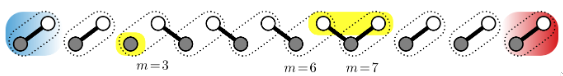
\includegraphics[width=0.85\textwidth]{fig/fig1-8.png}
    \caption{A long, fully dimerized SSH chain with 3 domains. The boundaries between the domains, the "domain walls", host zero energy eigenstates (yellow shading). These can be localized on a single site, as for the domain wall at $n=3$, or on a superposition of sites, as the odd superposition of the ends of the trimer shared between the $n=6$ and $n=7$ unit cell.}
    \label{fig:1.8}
\end{figure}

Consider a domain wall in an SSH system that is not in the fully dimerized limit.
The wavefunctions of the edge states at the domain walls will penetrate to some small depth in the bulk, with exponentially decaying evanescent tails.
For two domain walls at a distance of $M$ unit cells, the two edge states on the walls will hybridize form bonding and anti-bonding states.
At half filling, of these only the negative energy eigenstate will be occupied.
This state hosts a single electron, however, its wave function is localized with equal weight on the two domain walls.
Hence each domain wall, when well separated from other domain walls and the ends of the chain, will carry half an electronic charge.

\subsection{Exact Calculation of Edge States}\label{sec:1.5.6}
The zero energy edge states of the SSH model can also be calculated exactly, even in the \textbf{absence of translational invariance}.
Take the SSH model on $N$ unit cells,
\begin{equation}\label{eq:1.42}
    \hat{H} = \sum_{m=1}^N \left( v_m \dyad{m,B}{m,A} + h.c. \right) + \sum_{m=1}^{N-1} \left( w_m \dyad{m+1,A}{m,B} + h.c. \right)
\end{equation}
We are looking for zero energy eigenstate of the Hamiltonian
\begin{equation}\label{eq:1.43}
    \hat{H} \sum_{m=1}^N \left( a_m \ket{m.A} + b_m\ket{m,B} \right) = 0
\end{equation}
This gives $2N$ equations
\begin{equation}
    m = 1 \dots N-1: ~ ~ v_m a_m + w_m a_{m+1} = 0; ~ ~ w_m b_m + v_{m+1} b_{m+1} = 0 \label{eq:1.44}
\end{equation}
with boundary equation $v_N a_N = 0 $ and $v_1 b_1 = 0$.

This give the set of equations is solved by
\begin{equation}
    m = 2\dots N: ~ ~ a_m = \prod_{j=1}^{m-1} \frac{-v_j}{w_j}a_1 \label{eq:1.45}
\end{equation}
and
\begin{equation}
    m = 1\dots N-1: ~ ~ b_m = \frac{-v_N}{w_m} \prod^{N-1}_{j= m+1} \frac{-v_j}{w_j} b_N \label{eq:1.46}
\end{equation}
The boundar condition requires $b_1 = a_N = 0$.
This equations together say that in general case, there is no zoro energy eigenstate, $a_m = b_m = 0$.

In thermodynamic limit, $N\to \infty$, two approximaste solutions exist if the average intercell hopping is stronger that the intralcell hopping.
Defining the "bulk average values",
\begin{equation}
    \overline{\log \abs{v}} = \frac{1}{N-1} \sum_{m=1}^{N-1} \log \abs{v_m};~ ~ ~     \overline{\log \abs{w}} = \frac{1}{N-1} \sum_{m=1}^{N-1} \log \abs{w_m};  \label{eq:1.48}
\end{equation}
Then equation \eqref{eq:1.45} and \eqref{eq:1.46} translate to
\begin{equation}
    \abs{a_N} = \abs{a_1} e^{-(N-1)/\xi}; ~ ~ ~ \abs{b_1} = \abs{b_N} e^{-(N-1)/\xi} \frac{\abs{v_N}}{\abs{v_1}}  \label{eq:1.49}
\end{equation}
with the localization length
\begin{equation}
    \xi = \frac{1}{ \overline{\log{\abs{w}}} - \overline{\log{\abs{v}}} } \label{eq:1.50}
\end{equation}
If in the thermodynamic limit, the bulk average value \eqref{eq:1.48} make sense, and $\xi>0$, we have two approximate zero energy solutions,
\begin{equation}
    \ket{L} = \sum_{m=1}^N a_m \ket{m,A}; ~ ~ \ket{R} = \sum_{m=1}^N b_m \ket{m,B}  \label{eq:1.51}
\end{equation}
